\documentclass[paper=a4, fontsize=11pt]{scrartcl} 

\usepackage[T1]{fontenc} 
\usepackage[english]{babel}
\usepackage{amsmath,amsfonts,amsthm}

\usepackage{lipsum}

\usepackage{graphicx}
\usepackage{float}
  \floatplacement{figure}{H}
  \floatplacement{table}{H}
  
\usepackage{sectsty} 
\allsectionsfont{\centering \normalfont\scshape} 

\usepackage{fancyhdr} % Custom headers and footers
\pagestyle{fancyplain} % Makes all pages in the document conform to the custom headers and footers
\fancyhead{} % No page header - if you want one, create it in the same way as the footers below
\fancyfoot[L]{} % Empty left footer
\fancyfoot[C]{} % Empty center footer
\fancyfoot[R]{\thepage} % Page numbering for right footer
\renewcommand{\headrulewidth}{0pt} % Remove header underlines
\renewcommand{\footrulewidth}{0pt} % Remove footer underlines
\setlength{\headheight}{13.6pt} % Customize the height of the header

\usepackage[labelformat=empty]{caption}
\usepackage{color}
\usepackage{listings}
\lstset{ %
language=bash,                % choose the language of the code
basicstyle=\footnotesize,       % the size of the fonts that are used for the code
numbers=left,                   % where to put the line-numbers
numberstyle=\footnotesize,      % the size of the fonts that are used for the line-numbers
stepnumber=1,                   % the step between two line-numbers. If it is 1 each line will be numbered
numbersep=5pt,                  % how far the line-numbers are from the code
backgroundcolor=\color{white},  % choose the background color. You must add \usepackage{color}
showspaces=false,               % show spaces adding particular underscores
showstringspaces=false,         % underline spaces within strings
showtabs=false,                 % show tabs within strings adding particular underscores
frame=single,           % adds a frame around the code
tabsize=2,          % sets default tabsize to 2 spaces
captionpos=b,           % sets the caption-position to bottom
breaklines=true,        % sets automatic line breaking
breakatwhitespace=false,    % sets if automatic breaks should only happen at whitespace
escapeinside={\%*}{*)}          % if you want to add a comment within your code
}



\numberwithin{equation}{section} % Number equations within sections (i.e. 1.1, 1.2, 2.1, 2.2 instead of 1, 2, 3, 4)
\numberwithin{figure}{section} % Number figures within sections (i.e. 1.1, 1.2, 2.1, 2.2 instead of 1, 2, 3, 4)
\numberwithin{table}{section} % Number tables within sections (i.e. 1.1, 1.2, 2.1, 2.2 instead of 1, 2, 3, 4)

\setlength\parindent{0pt} % Removes all indentation from paragraphs - comment this line for an assignment with lots of text

%----------------------------------------------------------------------------------------
%	TITLE SECTION
%----------------------------------------------------------------------------------------

\newcommand{\horrule}[1]{\rule{\linewidth}{#1}} % Create horizontal rule command with 1 argument of height

\title{	
\normalfont \normalsize 
\textsc{Computational Science - ITB} \\ [25pt] % Your university, school and/or department name(s)
\horrule{0.5pt} \\[0.4cm] % Thin top horizontal rule
\small  Pengenalan Sains Komputasi - MonteCarlo\\ % The assignment title
%\horrule{2pt} \\[0.5cm] % Thick bottom horizontal rule
}

\author{\small{Ridlo W. Wibowo || 20912009}} % Your name

\date{\normalsize\today} % Today's date or a custom date

\begin{document}

\maketitle % Print the title

\large \textbf{Problem.}\\
Buatlah program untuk mengenerate bilangan random menggunakan algoritma \textit{Linear Congruential Generator} (LCG), lalu gunakan untuk menghitung integral tentu dari fungsi berikut ini:\\
\begin{equation*}
f(x) = \sqrt{1-x^{4}}
\end{equation*}
\begin{equation*}
f(x) = \sin(\sqrt x)
\end{equation*}
\begin{equation*}
f(x) = e^{x^{2}}
\end{equation*}

\vspace{2cm}
\large \textbf{Documentation.}\\
\textit{\textbf{Linear Congruential Generator}}\\
Generator ini merupakan contoh paling sederhana dari generator penghasil bilangan random. Perumusan yang digunakan adalah:
\begin{equation*}
r_{n+1} = (a \times r_{n} + c)\mod m,
\end{equation*} 
dengan\\
$r_{0} = $ seed\\
$r_{1}, r_{2}, r_{3}, ... = $ random numbers\\
$a, c, m$ are constants (multiplier, increment, and modulo)\\
Jika kita dapat memilih konstanta $a, c,$ dan $m$ di atas dengan teliti, maka kita akan mendapatkan generator bilangan random uniform antara $0$ hingga $m-1$.\\

Kekurangan dari LCG adalah $r_{n}$ dan $r_{n+1}$ tidak bebas sebagai bilangan random. Kita dapat memprediksi $r_{n+1}$ apabila $r_{n}$ diketahui, hal ini menyebabkan LCG tidak aman secara \textit{cryptography}. Namun LCG cukup bagus untuk pekerjaan selain berhubungan dengan keamanan, misalnya integrasi montecarlo, selain itu algoritmanya sangat mudah diterapkan dalam bahasa pemrograman.\\

Pemilihan konstanta untuk LCG dapat kita tentukan sendiri secara hati-hati, namun kita dapat mencoba menggunakan konstanta yang sudah biasa digunakan sebagai \textit{library} (walaupun ada library yang buruk, misalnya dari BSD, yang hingga akhirnya freeBSD mengubahnya, namun openBSD dan netBSD masih tetap menggunakannya). Beberapa telah dicoba, misalnya formula dari Microsoft berikut:
\begin{eqnarray*}
state_{n+1} &=& 214013 \times state_{n} + 2531011 (\mod 2^{31})\\
rand_{n} &=& state_{n} \div 2^{16}
\end{eqnarray*}
$rand_{n}$ berada pada rentang $0 - 32767$. Walaupun rentangnya kecil (resolusinya rendah) namun pengulangan sequencenya cukup besar, yakni akan terjadi setelah $2^{31} - 1$ (memungkinkan keluar angka yang sama namun sequencenya berbeda). Kemudian untuk membuat \textit{style} penggunaan bilangan random mirip yang digunakan pada bahasa C/C++ maka dibuat program header (\texttt{lcg.h}) sebagai berikut:
\lstset{frameround=fttt}
\begin{lstlisting}
/**********************************************/
/* linear congruential generator              */
/* copyleft (c). Ridlo W. Wibowo              */
/* based on Microsoft formula                 */
/**********************************************/
#ifndef LCG_H
#define LCG_H
#include <math.h>
#define MAX_RAND 32767

/* default seed */
static unsigned long int state = 1;

/* change seed */
void rseed(unsigned int s){
    state = s;
}
 
/* Linear Congruential Generator */
int randu(){
    unsigned int multiplier = 214013;
    unsigned int increment = 2531011;
    unsigned int modulo = pow(2,31);
    
    state = (state*multiplier + increment)%modulo;
    return state/pow(2,16);
}
#endif
\end{lstlisting}

\textbf{Tes penggunaan} (dibandingkan dengan fungsi \texttt{rand()} dari \texttt{stdlib.h})\\
\lstset{frameround=fttt}
\begin{lstlisting}
#include<iostream>
#include<stdlib.h>
#include<time.h>
#include "lcg.h"
using namespace std;

int main(){
    //srand(time(NULL));
    for (int i=0;i<5;i++){
        cout << rand() << endl;}

    //rseed(time(NULL));
    for (int i=0;i<5;i++){
        cout << randu() << endl;}

    return 0;
}
\end{lstlisting}

Hasil dua kali run, tanpa mengubah \textit{seed} (default).
\begin{verbatim}
ridlo@lockon-PC:~/kul/PengenalanSK/tugasRandomGen$ ./rn 
1804289383
846930886
1681692777
1714636915
1957747793

41
18467
6334
26500
19169
ridlo@lockon-PC:~/kul/PengenalanSK/tugasRandomGen$ ./rn 
1804289383
846930886
1681692777
1714636915
1957747793

41
18467
6334
26500
19169
\end{verbatim}

Hasil dengan mengubah seed berdasarkan waktu (\texttt{srand()} di \texttt{stdlib.h}, dan \texttt{rseed()} di \texttt{lcg.h}).
\begin{small}
\begin{verbatim}
ridlo@lockon-PC:~/kul/PengenalanSK/tugasRandomGen$ ./rn 
1458138624
1382823253
1777137677
705172191
2144641137

2315
25930
8873
2919
26891
ridlo@lockon-PC:~/kul/PengenalanSK/tugasRandomGen$ ./rn 
1005141763
446532302
731286527
914087325
1432220265

2331
14136
32658
24931
12927
\end{verbatim}
\end{small}

Jika kita bisa menggunakan \texttt{RAND\_MAX} di \texttt{stdlib.h} ($2147483647$), maka pengggantinya adalah \texttt{MAX\_RAND} di \texttt{lcg.h} di atas (32767). \\

\textbf{Tes \textit{randomness}} (untuk pasangan dua bilangan random).
\lstset{frameround=fttt}
\begin{lstlisting}
#include<iostream>
#include<fstream>
#include<time.h>
#include "lcg.h" // menggunakan fungsi random sendiri (microsoft)
using namespace std;

double unirand(){return (double)randu()/(double)MAX_RAND;} // rentang 0-1 

int main(){
    int N = 1000;
    rseed(time(NULL));
    ofstream out("random.txt");
    for (int i=0;i<N;i++){
        out << unirand() << " " << unirand() << endl;}
    out.close();    
    return 0;
}
\end{lstlisting}

\begin{figure}
	\centering
	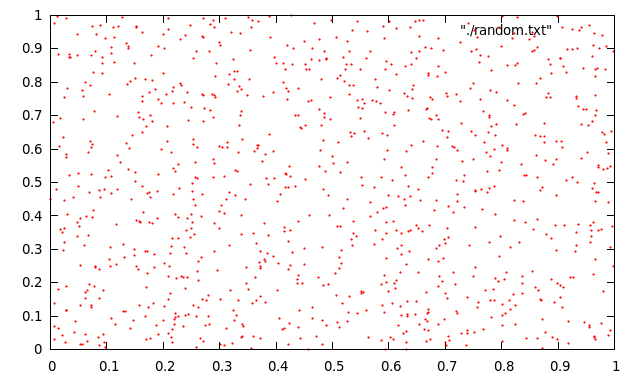
\includegraphics[width=0.8\textwidth]{1000.png}
	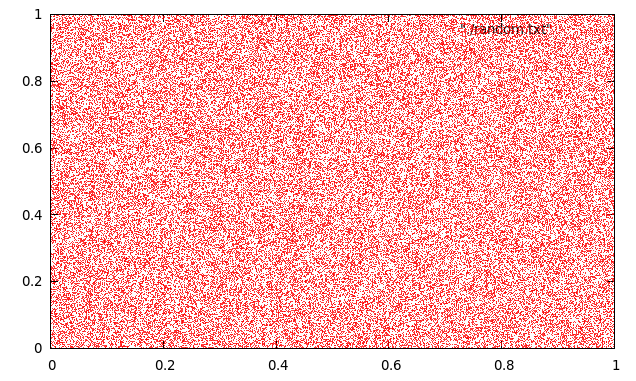
\includegraphics[width=0.8\textwidth]{100000.png}
	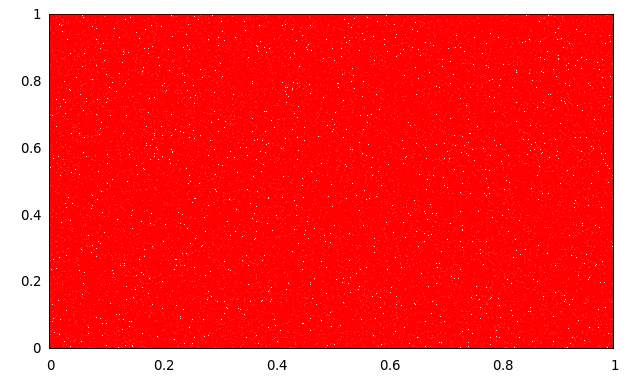
\includegraphics[width=0.8\textwidth]{1jt.png}
	\caption{$1000$, $10^{5}$, dan $10^{6}$ titik.}
\end{figure}

\textit{\textbf{Integral tentu dengan metode MonteCarlo}}\\
Seperti melempar darts, algoritma yang digunakan untuk menghitung integral tentu $1D$ dapat dibuat seperti berikut ini.\\
Algoritma:
\begin{enumerate}
\item Cari maksimum/minimum dari fungsi $f(x)$ (yaitu $c$) pada selang $a$ dan $b$ ($a$ dan $b$ adalah batas integrasi).
\item Lakukan hingga $N_{total}$:
	\begin{enumerate}
		\item random titik untuk $x$ dengan batas $a$ sampai $b$
		\item periksa apakah nilai $f(x)$ positif atau negatif
		\begin{itemize}
			\item Jika $f(x)$ positif :
			\begin{itemize}
				\item random untuk $y$ dengan batas $0$ sampai $c$.
				\item periksa apakah $y$ berada di bawah kurva $f(x)$, jika iya $N = N+1$
			\end{itemize}
			\item Jika $f(x)$ negatif :
			\begin{itemize}
				\item random untuk $y$ dengan batas $0$ sampai $-c$
				\item periksa apakah $y$ berada di atas kurva $f(x)$, jika iya $N = N-1$
			\end{itemize}
		\end{itemize}
	\end{enumerate}
\item $Hasil = \frac{N}{N_{total}} \times c \times (b-a)$
\end{enumerate}
dengan cara seperti di atas, kita dapat mengantisipasi apabila batas integrasi meliputi fungsi yang bernilai negatif (dapat dibuat untuk dimensi lebih tinggi pula). Pencarian nilai maksimum dapat juga dilakukan dengan cara menggunakan bilangan random (pendekatan).\\

\textbf{Untuk fungsi $f(x) = \sqrt{1-x^{4}}$}\\
- batas integrasi hanya diperbolehkan untuk $-1 \leq x \leq 1$.\\
- nilai maksimum di tentukan = 1 (program terlampir)\\

Hasil untuk $\int_{-1}^{1} \sqrt{1-x^{4}} dx$\\
Numerik = 1.748038369528061\\
Monte Carlo:
\begin{table}[ht]
\begin{tabular}{c c c c}
\hline
$run\_program$ & $N_{tot} = 10^{4}$ & $N_{tot} = 10^{5}$ & $N_{tot} = 10^{6}$  \\ [0.5ex]
\hline 
run\_01 & 1.739600 & 1.748760 & 1.749008 \\
run\_02 & 1.743200 & 1.748880 & 1.748966 \\
run\_03 & 1.745600 & 1.746940 & 1.746786\\
run\_04 & 1.745400 & 1.742600 & 1.746482\\
run\_05 & 1.748200 & 1.749440 & 1.747034\\ [0.5ex]
\hline 
average & 1.7444	 & 1.747324	& 1.7476552\\
\hline
stdev & 0.003215587	& 0.00280287	 & 0.0012314687\\
\hline
\end{tabular}
\end{table}

\textbf{Untuk fungsi $f(x) = \sin(\sqrt x)$}\\
- batas integrasi hanya untuk $x > 0$.\\
- nilai maksimum dicari dengan bilangan random (walaupun sudah jelas = 1) (program terlampir).\\

Hasil untuk $\int_{0}^{50} \sin(\sqrt x) dx$\\
Numerik = -8.557403169252579\\
Monte Carlo:
\begin{table}[ht]
\begin{tabular}{c c c c}
\hline
$run\_program$ & $N_{tot} = 10^{4}$ & $N_{tot} = 10^{5}$ & $N_{tot} = 10^{6}$  \\ [0.5ex]
\hline 
run\_01 & -8.068500 & -8.482650 & -8.668000 \\
run\_02 & -8.701000 & -8.485950 & -8.560695 \\
run\_03 & -8.827500 & -8.653150 & -8.569770\\
run\_04 & -8.503000 & -8.394650 & -8.625210\\
run\_05 & -7.920000 & -8.772500 & -8.602660\\ [0.5ex]
\hline 
average & -8.404	 & -8.55778	 & -8.605267\\
\hline
stdev & 0.395024841	& 0.1521640381	& 0.0435506865\\
\hline
\end{tabular}
\end{table}

\textbf{Untuk fungsi $f(x) = e^{x^{2}}$}\\
- batas integrasi hanya untuk $\vert x \vert < 26$ ($f(x)$ akan melebihi floating point).\\
- nilai maksimum dicari dengan f(x) pada batas terbesar (program terlampir).\\

Hasil untuk $\int_{-2}^{2} e^{x^{2}} dx$\\
Numerik = 32.905255531014461\\
Monte Carlo:
\begin{table}[ht]
\begin{tabular}{c c c c}
\hline
$run\_program$ & $N_{tot} = 10^{4}$ & $N_{tot} = 10^{5}$ & $N_{tot} = 10^{6}$  \\ [0.5ex]
\hline 
run\_01 & 32.2347 & 32.9358 & 32.9316 \\
run\_02 & 32.5623 & 33.2677 & 32.9847 \\
run\_03 & 32.0819 & 32.5602 & 32.9035 \\
run\_04 & 33.4141 & 33.0821 & 32.9768\\
run\_05 & 33.8945 & 32.6846 & 32.9275\\ [0.5ex]
\hline 
average & 32.8375 &	32.90608	 & 32.94482\\
\hline
stdev & 0.784179635 & 0.2878027571 & 0.0346237924\\
\hline
\end{tabular}
\end{table}

\newpage
\textbf{Diskusi}:
\begin{enumerate}
\item Semakin banyak jumlah titik random dan percobaan, maka semakin presisi hasil yang diperoleh (\textit{stdev} mengecil), walaupun tidak menjamin hasilnya lebih akurat.
\item Metode Monte Carlo akan mudah diterapkan untuk kasus integral lipat banyak (multiple integral).
\item Untuk permasalahan kompleks dapat dilakukan pembagian part integrasi dan melakukan perhitungan dengan menggunakan banyak komputer sekaligus (parallel computing).
\item Pelopor metode heuristic untuk memecahkan kasus-kasus lain.
\end{enumerate}

\vspace{1cm}
\textbf{Contoh \textit{run} dan \textit{error handling}}:\\
\begin{small}
\begin{verbatim}
ridlo@lockon-PC:~/kul/PengenalanSK/tugasRandomGen$ ./f2 
=== Definite Integral for f(x) = sin(sqrt(x))
=== using MonteCarlo method
Enter the boundary (x>=0):
Lower (a) = -2
Upper (b) = 50
N_total   = 10000
Error input boundary for this function
Enter the boundary (x>=0):
Lower (a) = 50
Upper (b) = 2
N_total   = 10000
Error input boundary for this function
Enter the boundary (x>=0):
Lower (a) = 0
Upper (b) = 50
N_total   = 10000
Hasil integrasi = -8.052000
ridlo@lockon-PC:~/kul/PengenalanSK/tugasRandomGen$ 
\end{verbatim}
\end{small}

\newpage
\textbf{Contoh plot} (untuk $\int_{0}^{50} \sin(\sqrt x) dx$) :\\
\begin{figure}
	\centering
	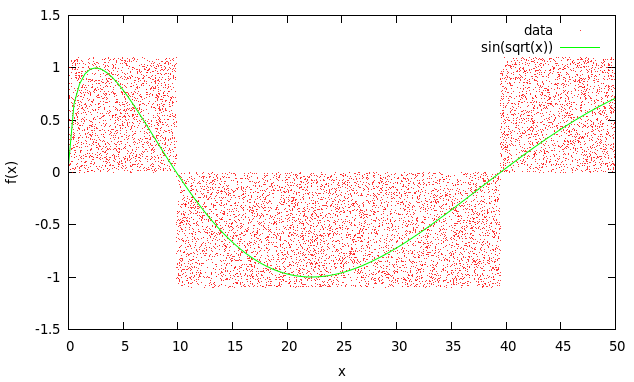
\includegraphics[width=0.7\textwidth]{f2-10rb.png}
	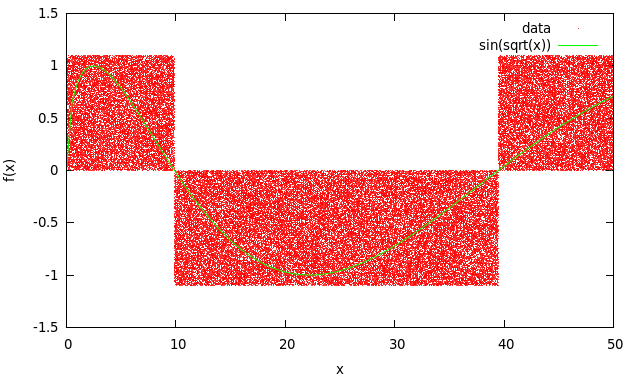
\includegraphics[width=0.7\textwidth]{f2-100rb.png}
	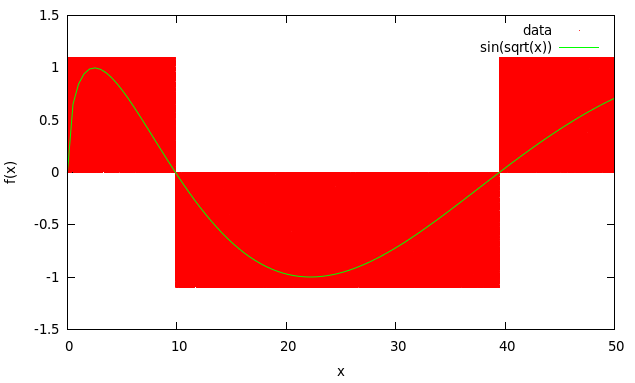
\includegraphics[width=0.7\textwidth]{f2-1jt.png}
	\caption{$10^{4}$, $10^{5}$, dan $10^{6}$ titik.}
\end{figure}

\newpage
\textbf{Lampiran}\\
Program tentunya menggunakan fungsi random yang sudah dibuat \texttt{lcg.h}.\\
\textit{f1.cpp}
\lstset{frameround=fttt}
\begin{lstlisting}
#include <iostream>
#include <stdio.h>
#include <math.h>
#include <time.h>
#include <fstream>
#include "lcg.h"
using namespace std;

int N, Ntot;
double x, y, res, a, b, c=1.0;

double unirand(){return (double)randu()/(double)MAX_RAND;}
double fx(double x){ return sqrt(1.-pow(x,4));}
void input();

int main(){
    cout << "=== Definite Integral for f(x) = sqrt(1-x^4)\n"; 
    cout << "=== using MonteCarlo method\n";    
    input();
    while (a < -1. || a > 1. || b < -1. || b > 1. || b < a || a == b){
        cout << "Error input boundary for this function\n";
        input();}
    
    // montecarlo
    rseed(time(NULL));
    ofstream out("f1-out.txt");
    for (int i=0;i<Ntot;i++){
        x = a + (b-a)*unirand();
        y = c*unirand();
        if (y<=fx(x)){ N++;}
        out << x << " " << y << endl;}
    out.close();
    res = (double)N/(double)Ntot * c * (b-a);
    printf("Hasil integrasi = %f\n", res);

    return 0;
}

void input(){   
    cout << "Enter the boundary (-1<=x<=1):\n";
    cout << "Lower (a) = "; cin >> a;
    cout << "Upper (b) = "; cin >> b;
    cout << "N_total   = "; cin >> Ntot;
}
\end{lstlisting}

\vspace{2cm}
\textit{f2.cpp}
\lstset{frameround=fttt}
\begin{lstlisting}
#include <iostream>
#include <stdio.h>
#include <stdlib.h>
#include <math.h>
#include <time.h>
#include <fstream>
#include "lcg.h"
using namespace std;

int N=0, Ntot=0;
double x, y, res, a, b, c=0.0;

double unirand(){return (double)randu()/(double)MAX_RAND;}
double fx(double x){ return sin(sqrt(x));}
void input();
void plot();

int main(){
    cout << "=== Definite Integral for f(x) = sin(sqrt(x))\n"; 
    cout << "=== using MonteCarlo method\n";    
    input();
    while (a < 0. || b < 0. || b < a || a == b || Ntot < 2){
        cout << "Error input boundary for this function\n";
        input();}
    
    // mencari maksimum dengan bilangan random
    for (int i=0;i<Ntot;i++){
        x = a + (b-a)*unirand();
        if (fabs(fx(x)) > c) {c = fabs(fx(x));}}
    c = c + 0.1; // agar lebih menjamin c >= maksimum fungsi

    // montecarlo
    rseed(time(NULL));
    ofstream out("f2-out.txt");
    for (int i=0;i<Ntot;i++){
        x = a + (b-a)*unirand();
        if (fx(x) >= 0.){
            y = c*unirand();
            if (y <= fx(x)){ N++; }}
        else {
            y = -c*unirand();
            if (y >= fx(x)){ N--; }}
        out << x << " " << y << "\n";
    }
    out.close();
    
    res = ((double)N / (double)Ntot) * c * (b-a);
    printf("Hasil integrasi = %f\n", res);

    plot();
    return 0;
}

void input(){   
    cout << "Enter the boundary (x>=0):\n";
    cout << "Lower (a) = "; cin >> a;
    cout << "Upper (b) = "; cin >> b;
    cout << "N_total   = "; cin >> Ntot;
}

void plot(){
    ofstream ploter("plot.in");
    ploter << "#gnuplot input file\n";
    ploter << "set xlabel \"x\"\n";
    ploter << "set ylabel \"f(x)\"\n";
    ploter << "plot \"f2-out.txt\" w d title \"data\", sin(sqrt(x)) w l\n";
    ploter.close();
    
    system("gnuplot -persist < plot.in");
}
\end{lstlisting}

\vspace{2cm}
\textit{f3.cpp}
\lstset{frameround=fttt}
\begin{lstlisting}
#include <iostream>
#include <stdio.h>
#include <math.h>
#include <time.h>
#include <fstream>
#include "lcg.h"
using namespace std;

int N, Ntot;
double x, y, res, a, b, c;

double unirand(){return (double)randu()/(double)MAX_RAND;}
double fx(double x){ return exp(x*x);}
void input();

int main(){
    cout << "=== Definite Integral for f(x) = exp(x^2)\n"; 
    cout << "=== using MonteCarlo method\n";    
    input();
    while (a < -26. || a > 26. || b < -26. || b > 26. || b < a || a == b){
        cout << "Error input boundary for this function\n";
        input();}
    
    // maksimum mengambil batas, karena fungsi selalu positif
    c = fabs(fx(b));
    if (fabs(b) < fabs(a)){ c = fabs(fx(a));}

    // montecarlo
    rseed(time(NULL));
    ofstream out("f3-out.txt");
    for (int i=0;i<Ntot;i++){
        x = a + (b-a)*unirand();
        y = c*unirand();
        if (y<=fx(x)){ N++;}
        out << x << " " << y << endl;}
    out.close();
    res = (double)N/(double)Ntot * c * (b-a);
    printf("Hasil integrasi = %g\n", res);

    return 0;
}

void input(){   
    cout << "Enter the boundary (-26<=x<=26):\n";
    cout << "Lower (a) = "; cin >> a;
    cout << "Upper (b) = "; cin >> b;
    cout << "N_total   = "; cin >> Ntot;
}
\end{lstlisting}
\end{document}














